\documentclass[../main.tex]{subfiles}
\graphicspath{{\subfix{../images/}}}
\begin{document}
\section{Entwicklung}

\subsection{Hardware}
\subsubsection{Bridge}
Zur Entwicklung der Verbindungsplatine wurde die Hardware zunächst auf einem Breadboard aufgesteckt und eine geeignete Verbindung der notwendigen Pins mithilfe ausreichender Steckbrückenkabel hergestellt und umfangreich getestet. Anschließend wurde der Schaltplan nach Vorlage des Breadboards in KiCad Version 7.0 erstellt, woraus sich im weiteren Verlaufe ein Leiterplattenentwurf erstellen ließ. Der Druck der Leiterplatte erfolgte auf Anfrage im KI-Labor am Umwelt-Campus Birkenfeld.

\begin{figure}[!ht]
    \centering
    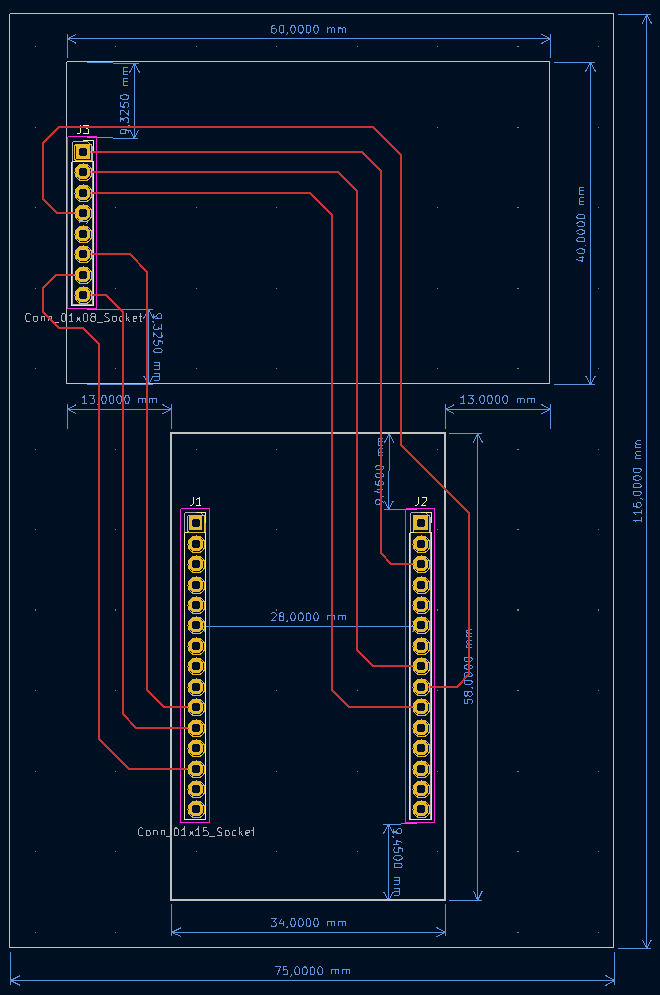
\includegraphics[width=0.4\textwidth, angle=-90]{images/leiterplatte.png}
    \caption{Leiterplattenplan aus dem Leiterplatteneditor der Software KiCad 7}
    \label{fig:Bridge}
    \centering
\end{figure}



\subsubsection{Hülle}

Das Gehäuse wurde innerhalb von Fusion 360 designt und dann mit PLA Filament 3D gedruckt. Es hat mehrere Anläufe gebraucht um das richtige Design hinzubekommen.

\begin{figure}[!ht]
    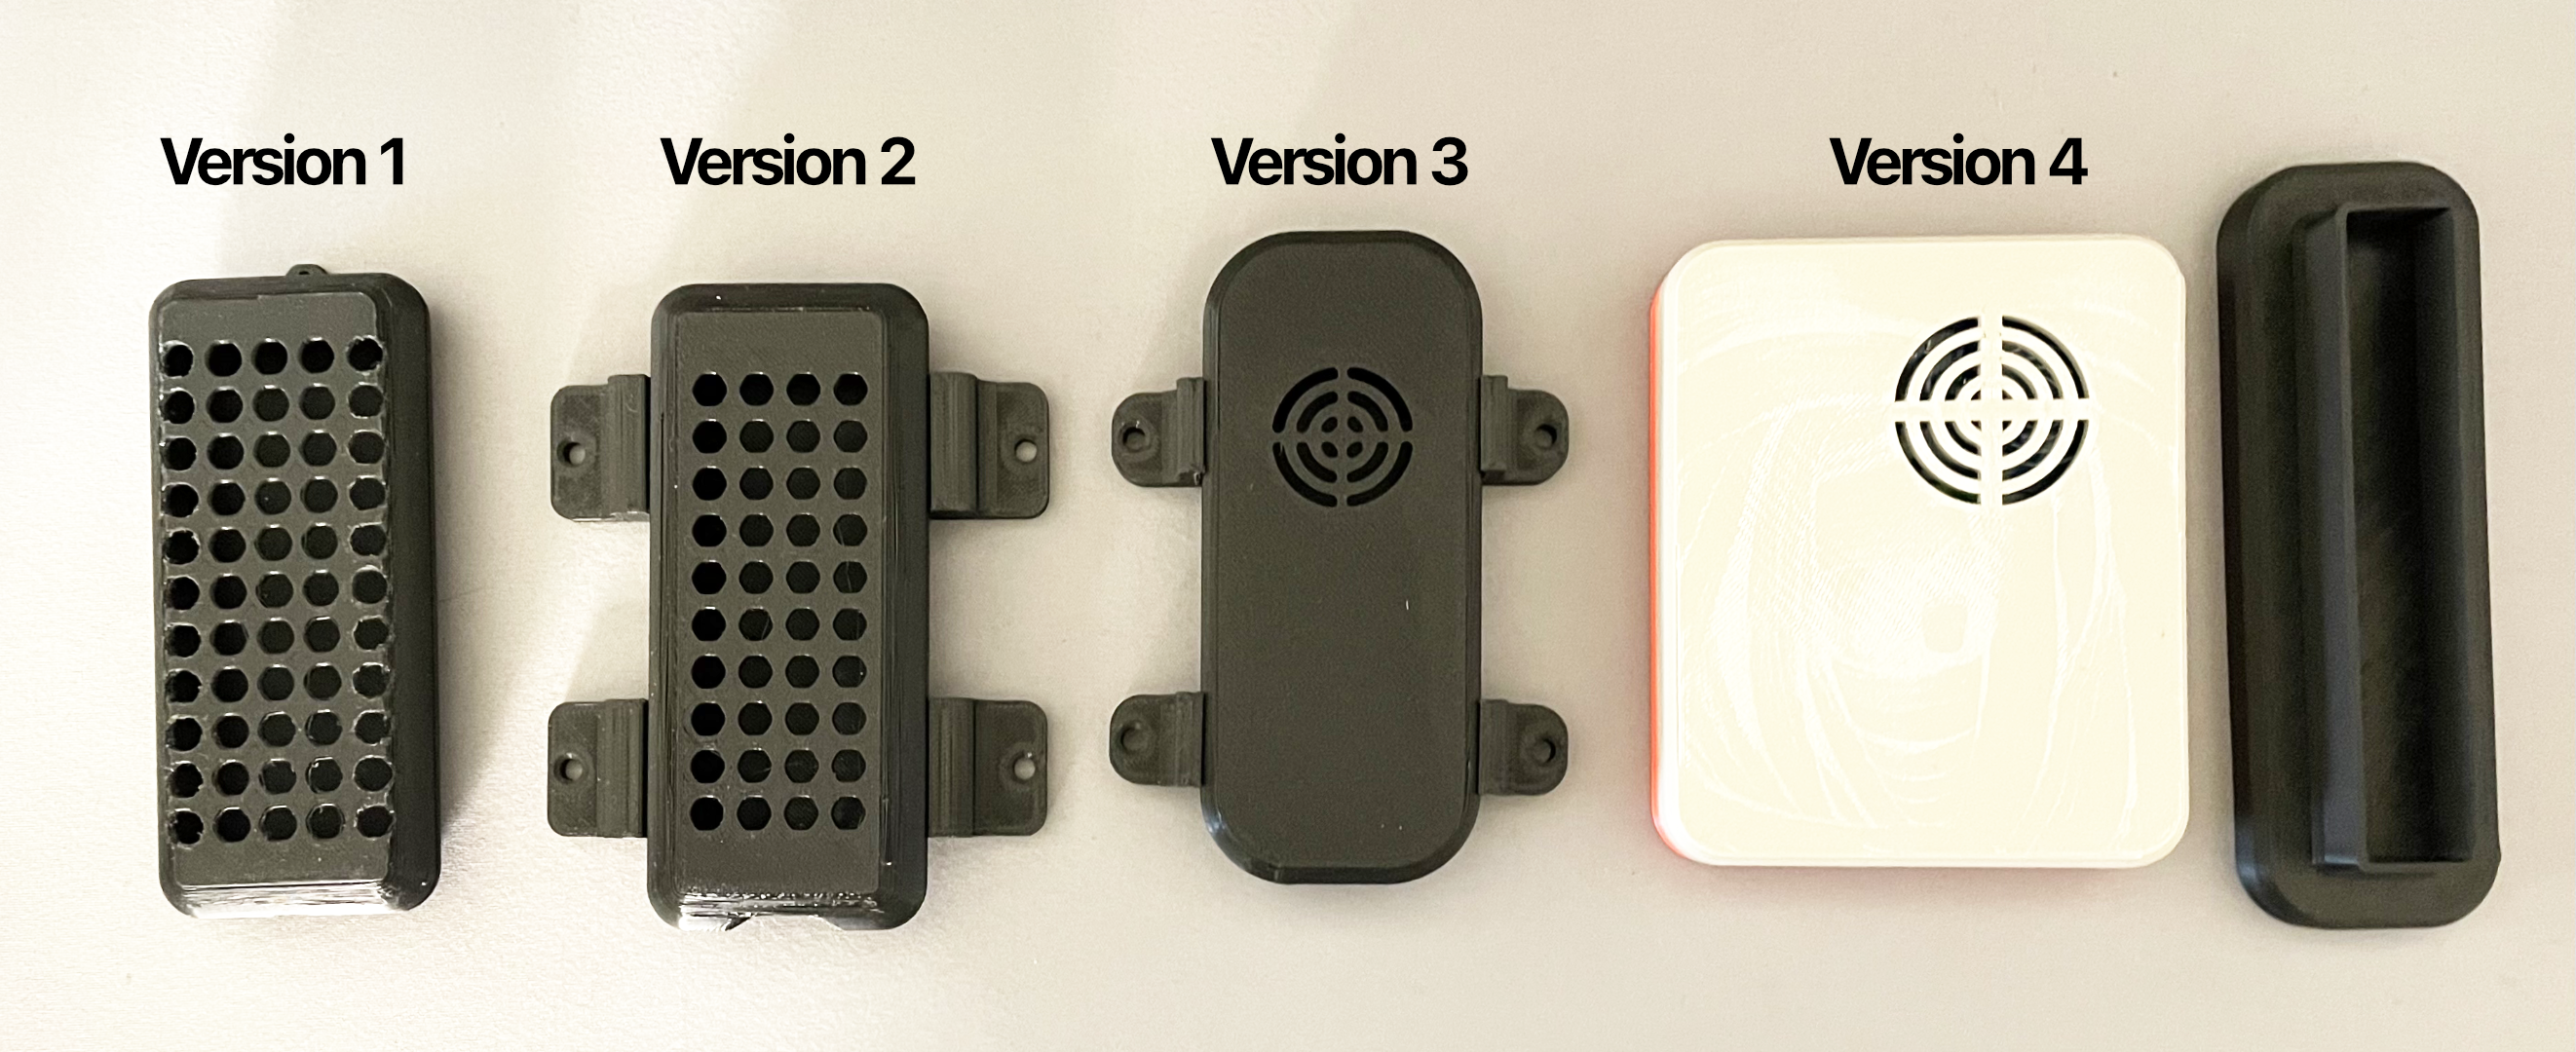
\includegraphics[width=\linewidth]{images/huellen_versionen.png}
    \caption{Alle Versionen des Hüllendesigns}
    \centering
\end{figure}

\subsection{API Design} \label{JSON-API}

Zur Erstellung unseres Systems haben wir uns auf folgende JSON Struktur geeinigt, um die Daten zwischen den verschiedenen Softwaresystemen zu kommunizieren. 

\begin{lstlisting}
{
    "key": "api key",
    "data": {
        "request_data": "Some Data"
    },
    "error": "Error Message"
}
\end{lstlisting}

\begin{itemize}
  \item\textbf{Key}: Das Key Attribut enthält den API-Schlüssel, welcher das System schützt vor nicht autorisierten Zugriffen.
  \item\textbf{Data}: Ist ein weiteres JSON Objekt innerhalb der Abfrage, welches Abfragen spezifische Daten enthält.
  \item\textbf{Error}: Error enthält den Text einer entstandenen Fehlermeldung.
\end{itemize}

\subsection{Benutzeroberfläche}

Die Umsetzung der Benutzeroberfläche für unser Zeitverwaltungssystem wurde durch die Anwendung der Template Engine Pug realisiert, welche eine effiziente und elegante Möglichkeit bietet, HTML-Dateien zu generieren. Zur Gestaltung der Bedienelemente griffen wir auf Bootstrap zurück, eine bewährte Bibliothek für responsives Design und eine Vielzahl von vorgefertigten Komponenten. Darüber hinaus ermöglichte uns Alpine.js, dynamische Inhalte auf den Seiten nahtlos zu ändern und eine interaktive Benutzererfahrung zu schaffen. 
Wir haben versucht, ein einheitliches Design über die Seiten verteilt zu verwenden. Auf der Startseite hat man eine Übersicht über alle Ein/-Abmeldungen. Für die Punkte, Nutzern, Karten und Positionen gibt es jeweilige Listen und Detailansichten. Um Daten anzulegen oder zu verändern, gibt es die passenden Formulare. Um Daten zu löschen, gibt es eine einheitliche Seite zur Bestätigung der Aktion. Das Farbschema ist bewusst irreführend gewählt, damit ein Nutzer länger braucht, um die Aktion zu vollenden, um fehl Entscheidungen zu minimieren.

\subsection{Datenverwaltung/Datenbearbeitung}

Nutzerdaten werden innerhalb der Webformulare erstellt und dann via den Control Schnittstellen in eine SQLite Datenbank eingetragen. Die Formulardaten werden via POST Request an die Route zurückgegeben und dort werden die Daten weiter gegeben an den Controller, der letztlich die richtige Funktion auf unserem Modell ausführt. Dieses Modell ist eine Abstraktion von unserer SQL Datenbank, welche die Entwicklung erleichtert und durch seine einheitlichen Schnittstellen Fehler verhindert. Die Modelle können alle CRUD Operationen ausführen auf dem Modell, Funktionsweisen, welche komplexer sind, sollten von Controller übernommen werden, um unnötige Komplexität zu verhindern.

\begin{figure}[!ht]
    \centering
    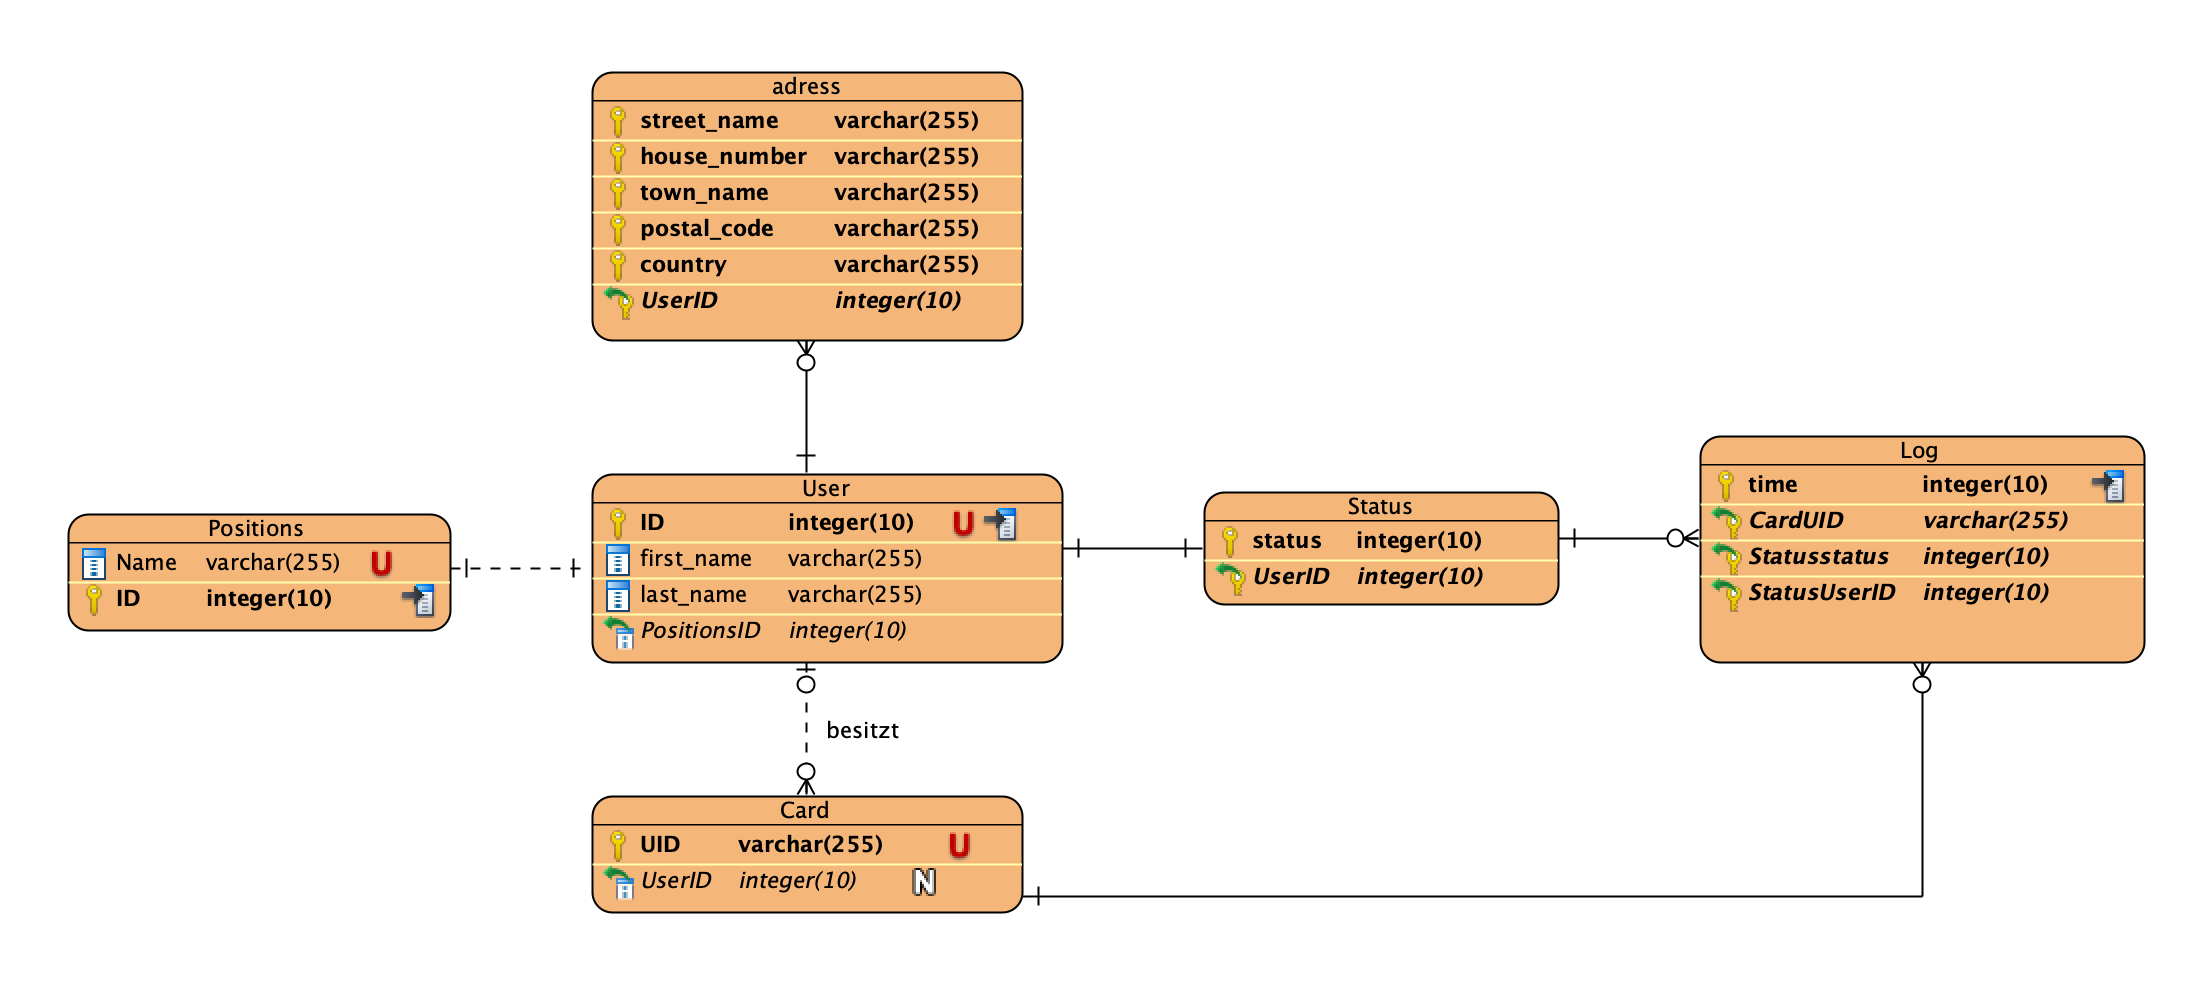
\includegraphics[width=0.75\textwidth]{images/Datenbank Modell.png}
    \caption{Entity Relationship Diagramm}
    \label{fig:ER}
    \centering
\end{figure}

\subsection{Zeiterfassung} \label{ZeitwerfassungEntwicklung}
Zunächst wurden Nachforschungen betrieben, welche Möglichkeiten es gibt, um eine zuverlässige Erfassung der Zeit zu gewährleisten. Neben diversen hardwarebasierten Erfassungsmethoden fiel Wahl schließlich auf eine softwarebasierte Erfassung. Dies umfasst die Zeitanfrage über eine Anfrage an einen Network Time Protokoll Server.\\
Der Vorteile, der sich hieraus ergibt, ist, dass keine weitere Hardware benötigt wird, um die Zeit zu erfassen.\\ 
Der größte Nachteil dieser Methode ist jedoch, dass zwangsläufig eine Netzwerkverbindung bestehen muss, um die Zeit vom NTP Server erhalten zu können.
\subsubsection{Unix Epoch Time} 
Die Zeit wird hierbei lediglich als Unix Timestamp, also der Anzahl an vergangenen Sekunden seit dem 1. Januar 1970, 00:00 Uhr UTC, erfasst und an den Server weitergegeben, da die Zeit dadurch einfach als Integer in der Datenbank hinterlegt werden kann. Hier kommt es jedoch zu Komplikationen der Zeiterfassung am 19. Januar 2038, da unsere Datenbank lediglich 32-Bit Integer speichert.

% Was ist der Unterschied von Datenanzeige und Darstellung

\subsection{Sicherheit}

Um sicherzustellen, ob ein Zeiterfassungsgerät (ESP) auf den Server zu greifen darf, wird bei jeder Anfrage ein Schlüssel mitgegeben, der bei jeder „log“ Anfrage überprüft wird.

\subsection{Protokollierung}

Wenn ein Nutzer eine RFID Karte an das Lesegerät hält, erfasst der ESP die UID in der Karte. Danach macht der ESP eine POST Anfrage an den Server. Danach trägt der Server den erzeugten Eintrag in die Log-Tabelle. Ein Eintrag besteht aus der Epoch time der Karten UID, dem zu gehörigen User und den veränderten Status.

\end{document}